\Section{naturalli}{Improving Inference in NaturalLI}
% Overview paragraph
We extend NaturalLI in a few key ways to improve its coverage for question
  answering tasks over complex sentences.
We adapt the search algorithm to operate over dependency
  trees, rather than the surface form of the sentence (\refsec{naturalli-trees}).
We enrich the class of inferences warranted by natural logic beyond
  hypernymy and operator rewording to also encompass meronymy and
  relational entailment (\refsec{naturalli-meronym}).
Lastly, we handle token insertions during search more elegantly
  (\refsec{naturalli-forward}).

% Three search operations
The general search algorithm in NaturalLI is parametrized as follows:
First, an order is chosen to traverse the tokens in a sentence.
For example, the original paper traverses tokens left-to-right.
At each token, one of three operations can be performed:
  these are \textit{deleting} a token
  -- corresponding to inserting a word during natural logic inference,
  \textit{mutating} a token, and \textit{inserting} a token -- again, corresponding
  to deleting a token in the forward entailment.
For brevity, we will refer to an insertions during inference (deletions during
  search) as \textit{deletions}, and vice versa for insertions.

%
% Dependency Trees
%
\Subsection{naturalli-trees}{Natural logic over Dependency Trees}
Operating over dependency trees rather than a token sequence requires reworking
  (1) the semantics of deleting a token during search, and 
  (2) the order in which the sentence is traversed.

%% Zoom in on what we're changing
%We handle this last operation outside of the search procedure (see \refsec{naturalli-forward}),
%  and turn our attention to the first two.
%Mutating a token in turn remains unchanged, beyond the addition of new inference rules
%  (see \refsec{naturalli-meronym}).
%This leaves us to define the semantics of deleting tokens during the search, and
%  deciding an order in which to traverse the tokens.

% Talk about deletion
Recent work by \newcite{key:2015angeli-openie} defined a mapping from Stanford
  Dependency relations to the associated lexical relation deleting the
  dependent subtree would induce.
%For instance, deleting an \textit{amod} edge induces \forward\ -- it maintains
%  entailment in an upward polarity context.
We adapt this mapping to yield the relation induced by \textit{inserting} a
  given dependency edge, corresponding to our deletions in search;
%  (recall, a deletion during search is an insertion during
%  inference); 
  we also convert the mapping to use Universal Dependencies
  \cite{key:stanford-ud}.
This now lends a natural deletion operation: at a given node, the subtree rooted
  at that node can be deleted to induce the associated natural logic relation.

% Example of deletion
For example, we can infer that 
  \w{all truly notorious villains have lairs} from the premise
  \w{all villains have lairs} by observing that deleting
  an \textit{amod} arc induces the relation \reverse, which in the downward
  polarity context of \textit{\tagDown{villains}} projects to \forward\ (entailment):

\begin{center}
\begin{dependency}[text only label, label style={above}]
  \begin{deptext}[column sep=-0.00cm]
    \tagUp{All} \& \tagDown{truly} \& \tagDown{\darkred{notorious}} \& 
      \tagDown{villains} \& \tagUp{have} \& \tagUp{lairs} \&[-1ex] .\\
  \end{deptext}
  \depedge[edge unit distance=1.0ex]{5}{1}{operator}
  \depedge[edge unit distance=1.25ex]{5}{4}{nsubj}
  \depedge[edge unit distance=1.25ex, edge style={darkred!100!black,thick}]{4}{3}{\darkred{amod}}
  \depedge[edge unit distance=1.25ex, edge style={darkred!100!black,thick}]{3}{2}{advmod}
  \depedge[edge unit distance=1.25ex]{5}{6}{dobj}
\end{dependency}
\end{center}

% Talk about ordering
This leaves the question of the order to traverse the token in the sentence.
The natural order is to perform a breadth-first traversal of the dependency tree.
This avoids repeated deletion of nodes, as we do not have to traverse any
  subtree which has been deleted.

% Subtlety about operators
A subtlety to consider here is the effect mutating an operator has on the
  polarity of its arguments -- for example, mutating \w{some} to
  \w{all}.
There are cases where we must mutate the argument to the operator before
  the operator itself, as well as cases where we must mutate the operator
  before its arguments.
Consider, for instance:

\entailmentExample
{All felines have a tail}
{Some cats have a tail}

\noindent where we must first mutate \w{cat} to \w{feline}, contrasted with:

\entailmentExample
{All cats have a tail}
{Some felines have a tail}

\noindent where we must first mutate \w{some} to \w{all}.
Therefore, our traversal first visits each operator, then performs a breadth-first
  traversal of the tree, and then visits each operator a second time.

%
% Meronymy
%
\Subsection{naturalli-meronym}{Meronymy and Relational Entailment}
%
% Parital Orders Figure
%
\begin{figure*}
\begin{center}
\begin{tabular}{ccc}
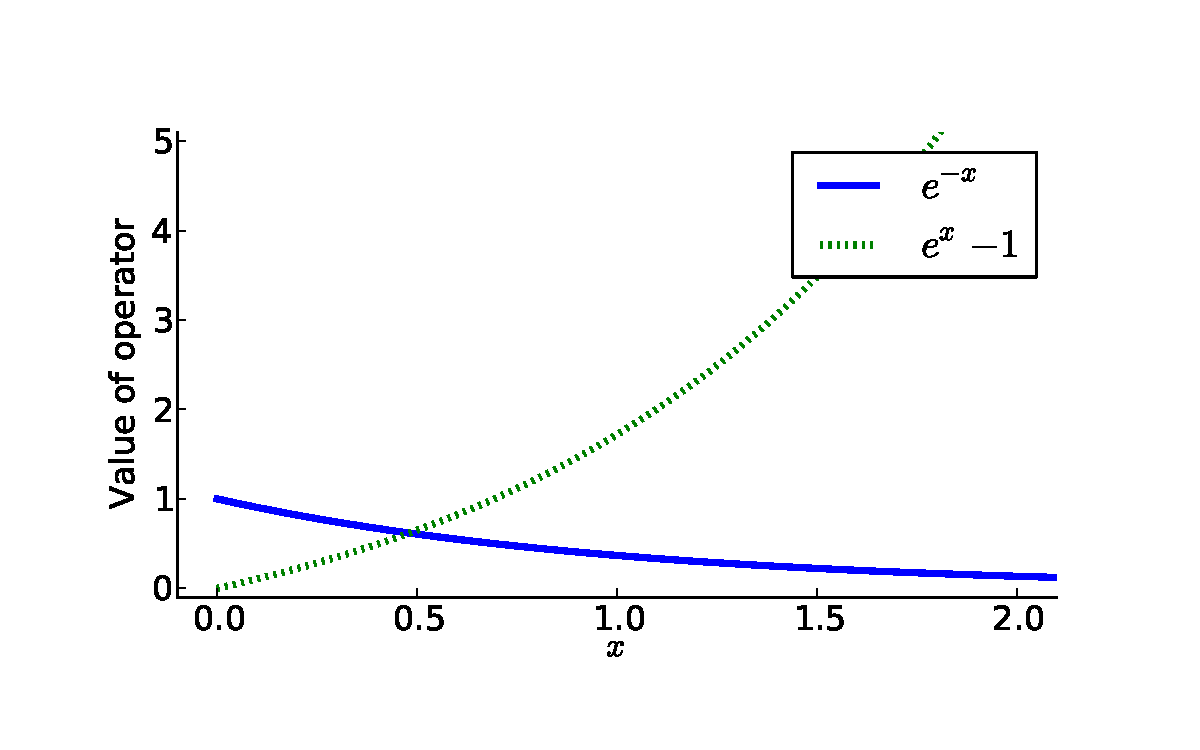
\includegraphics[scale=0.27]{../img/monotonicity_math.pdf} &
\hspace{-2em}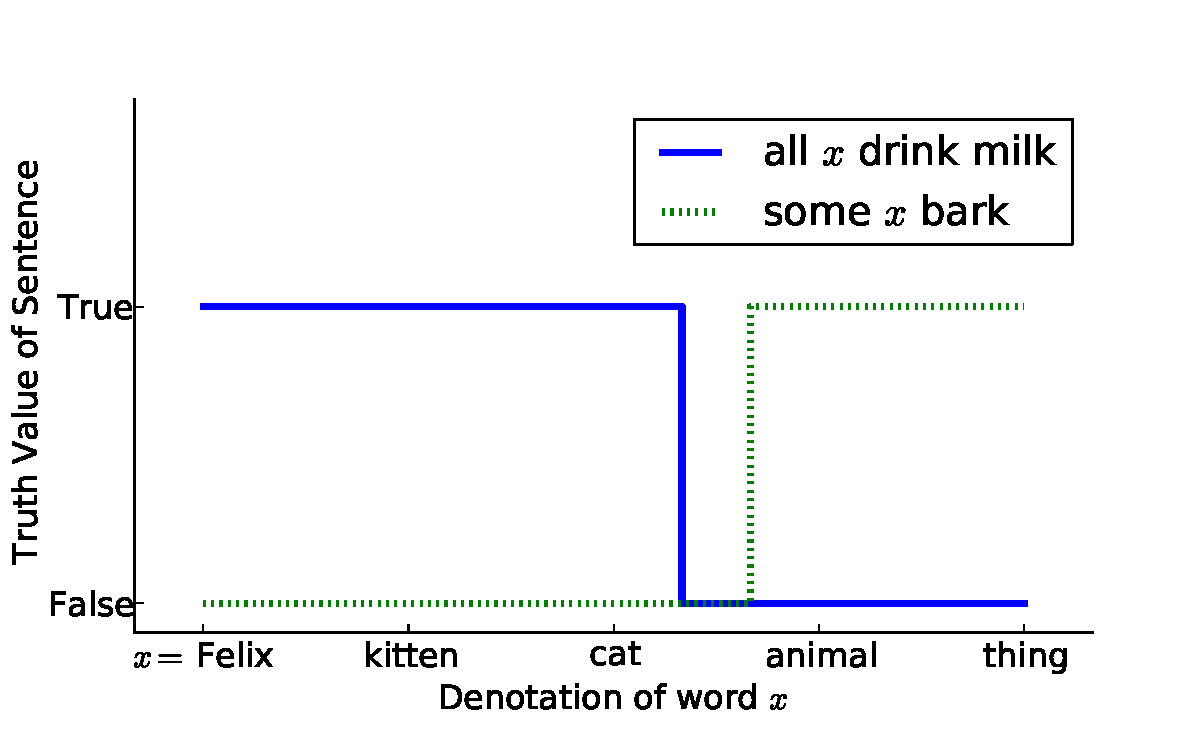
\includegraphics[scale=0.27]{../img/monotonicity_lex_all.pdf} &
\hspace{-2em}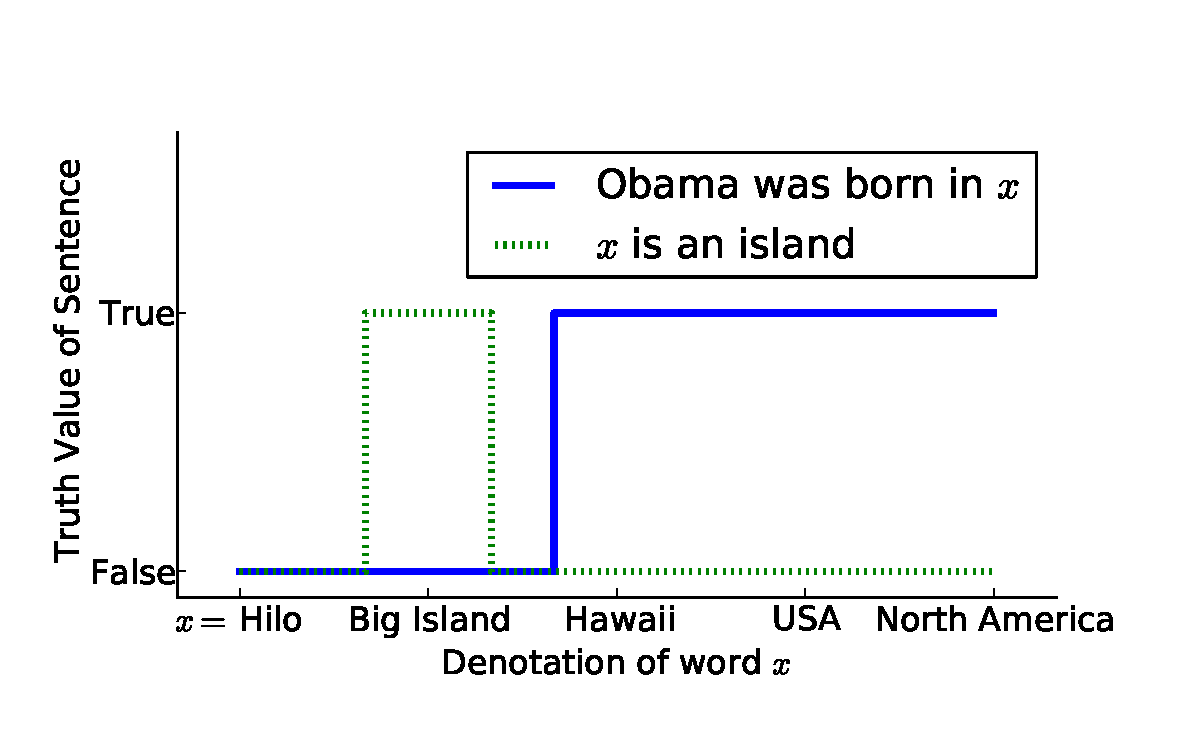
\includegraphics[scale=0.27]{../img/monotonicity_lex_meronymy.pdf}\\
(a) & (b) & (c)
\end{tabular}
\end{center}
\caption{
An illustration of monotonicity using different partial orders.
(a) Monotonicity illustrated over real numbers: $e^x-1$ is monotone whereas
    $e^{-x}$ is antitone.
(b) The monotonicity of \w{all} and \w{some} in their first arguments, over
    a domain of denotations.
(c) An illustration of the \w{born in} monotone operator over the meronymy hierarchy,
    and the operator \w{is an island} as neither monotone or antitone.
}
\end{figure*}

% Cute example of partial orders
Although natural logic and the underlying monotonicity calculus has 
  only been explored in the context of hypernymy, the underlying framework
  can be applied to any partial order over lexical items.
To give a simple example, 
  we can consider a natural logic over integers \cite{key:2014icard-natlog}.
%  -- which have a total, and therefore partial order.
If we observe that the numeric operator $e^{-x} : \bR \rightarrow \bR$ is
  antitone, then we can infer that because $2 \geq 1$ (i.e., $2 \reverse 1$)
  we know that $e^{-2} \leq e^{-1}$ (i.e., $e^{-2} \forward e^{-1}$), without
  ever evaluating the operator $e^{-x}$ explicitly.

% Translate to language
In the same way, natural language operators are defined as a mapping from
  denotations of objects, to truth values.\footnote{
  Truth values are a trivial partial order corresponding to entailment:
  if \hbox{$t_1 \leq t_2$} 
  (i.e., \hbox{$t_1 \forward t_2$}),
  and you know that $t_1$ is true, then $t_2$ must be true.
}
%The domain of word denotations is then ordered by the subset operator, corresponding
%  to ordering by hypernymy over the words.
% New partial orders
However, hypernymy is not the only useful partial ordering over denotations.
We include two additional orderings as motivating examples: relational
  entailment and meronymy.

% Relational entailment
\paragraph{Relational Entailment}
For two verbs $v_1$ and $v_2$, we define $v_1 \leq v_2$ if the first verb
  entails the second.
This entailment judgment can be gathered from an external resource, such as
  \textsc{VerbOcean} \cite{key:2004chklovski-verbocean}.
%In many cases, these entailments are not hypernymy.
In many cases, a verb $v_1$ may entail a verb $v_2$ even if $v_2$ is not a hypernym of $v_1$.
For example, to \w{sell} something (hopefully) entails \w{own}ing that thing.
Apart from esoteric context-specific cases (e.g., \w{orbit} entails \w{launch} only
  for man-made objects), these relations hold largely independent of context.
%Note that the usual operators apply to relational entailments -- if 
%  \w{all cactus owners live in Arizona} then \w{all cactus sellers live in Arizona}.

Verb entailment information was incorporated using data from \textsc{VerbOcean}
 \cite{key:2004chklovski-verbocean}, adapting the confidence weights as costs.
\textsc{VerbOcean} uses lexicosyntactic patterns to score pairs of verbs as candidate participants in a set of relations.
%We approximate the \textsc{VerbOcean} relations $\mathit{stronger \mhyphen than}(v_1,v_2)$ and $\mathit{happens \mhyphen before}(v_2,v_1)$ to indicate that $v_1$ entails $v_2$.
We approximate the \textsc{VerbOcean} relations $\mathit{stronger\text{-}than}(v_1,v_2)$ and $\mathit{happens\text{-}before}(v_2,v_1)$ to indicate that $v_1$ entails $v_2$.
%These verb entailment transitions are incorporated using costs derived from the original weights from \newcite{key:chklovski2004verbocean}, after thresholding as indicated in the original paper. 

% Meronymy
\paragraph{Meronymy}
The most salient use-case for meronymy is with locations.
For example, if Obama was born in Hawaii, then we know that Obama was born in
  America, because Hawaii is a meronym of (part of) America.
Unlike relational entailment and hypernymy, meronymy is operated on by a
  distinct set of operators:
  if \w{Hawaii is an island}, we cannot necessarily entail that \w{America
  is an island}.
We collect a set of operators which are either monotone or antitone with respect
  to the meronymy hierarchy (e.g., \w{born in}, \w{visited}); 
  these then compose in the usual way with the conventional 
  operators (e.g., \w{some}, \w{all}).

We use a set of 81 triggers for meronymy, which were manually labeled as monotonic or antitonic. These triggers consist of dependency paths of length 2 that co-occurred in newswire text with a named entity of type \w{PERSON} and two different named entities of type \w{LOCATION}, such that one location was a meronym of the other.

Meronymy transitions are drawn from instances of the relation \texttt{location-contains} in Freebase \cite{key:2008bollacker-freebase}.
This relation exists between entities of type \textit{location} in Freebase, where one location exists completely within the boundaries of the other location.
%As this relation is also based on an underlying partial order, 
We are able to use a weighting scheme analogous to that used for the hypernymy transitions.
%We also instantiate the inverse, holonymy transitions.

%% Other orders
%Note that these are not the only two orders that can be incorporated into our
%  framework; they just happen to be two which have lexical resources available
%  and are likely to be useful in real-world entailment tasks.

%
% Forward Search
%
\Subsection{naturalli-forward}{Removing the Insertion Transition}
% Review Trie
%Deleting tokens in a natural logic inference manifest as inserting tokens
%  during search.
Inserting words during search poses an inherent problem, 
  as the space of possible words to insert at any
  position is on the order of the size of the vocabulary.
In NaturalLI, this was solved by keeping a trie of possible insertions, and
  using that to prune this space.
However, this is both computationally slow and adapts awkwardly to a search over
  dependency trees.

% Pre-compute deletion
Therefore, this work instead opts to perform a bidirectional search:
  when constructing the knowledge base, we add not only the original sentence but
  also all entailments with subtrees deleted.
For example, a premise of \w{some furry cats have tails} would yield two facts
  for the knowledge base: \w{some furry cats have tails} as well as \w{some cats
  have tails}.
%For this, we use the process described in \newcite{key:2015angeli-openie} to
%  generate short entailed sentences from a long utterance using natural logic.
%This then leaves the reverse search to only deal with mutations and inference  
%  insertions, which are relatively easier.

% Difficulties
The additional challenge this introduces, of course, is the additional space required
  to store the new facts.
To mitigate this, we hash every fact into a 64 bit integer, and store only the hashed 
  value in the knowledge base.
We construct this hash function such that it operates over a bag of edges in the
  dependency tree -- in particular, the XOR of the hash of each dependency edge in
  the tree.
This has two key properties: it allows us to be invariant to the word order of
  of the sentence, and more importantly it allows us to run our search directly
  over modifications to this hash function.

% Elaborate on search over hash function
To elaborate, we notice that each of the two classes of operations our search is
  performing are done locally over a single dependency edge.
When adding an edge, we can simply take the XOR of the hash saved in the 
  parent state and the hash of the added edge.
When mutating an edge, we XOR the hash of the parent state with the edge we are
  mutating, and again with the mutated edge.
% Sad to cut -- so much coding time unappreciated :(
%In this way, each search node need only carry an 8 byte hash, local information
%  about the edge currently being considered (8 bytes), global information about the words
%  deleted during search (5 bytes), a 3 byte backpointer to recover the
%  inference path, and 8 bytes of operator metadata -- 32 bytes in all.
%This results in an incidental contribution of having made NaturalLI significantly
%  faster and more memory efficient.

